% Chapter 3

\chapter{System Architecture}
\label{Chapter3}
\lhead{Chapter 3. \emph{System Architecture}}

\section{Overview}
IronClaw is an autonomous-agent hosting platform that has a very strict host / guest split. The host process (daemons), ironclawd, is responsible for all of the "privileged" things in the system; these include loading the configuration file, enforcing policies, managing memory, interacting with large language models (LLM), and controlling the lifecycle of micro-VMs. The guest runtime, irowclaw, is executing within a Firecracker boundary and will execute untrusted tool requests coming from the host.

This design was intended to be asymmetric. The host is assumed to be trusted and stateful: it maintains the conversation state, holds onto long-term configurations, makes decisions about what tools are allowed, and retains connections to external model providers. Conversely, the guest is intentionally small and ephemeral: it accepts bounded executions on behalf of the host, run those executions against a set of policies, returns structured data back to the host and can be discarded once it's completed its task. This separation allows the complex logic for controlling agents to exist in a trusted location away from the potentially un-trusted execution environment while also prevents synthesized tools from being able to access resources held by the host workspace.

\begin{figure}[htbp]
    \centering
    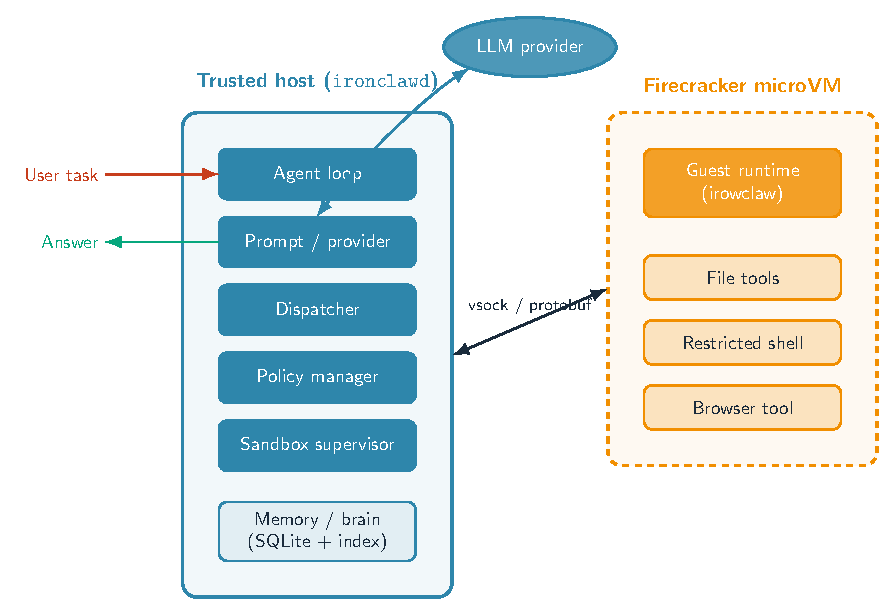
\includegraphics[width=0.95\linewidth]{Figures/fig_architecture.pdf}
    \caption{IronClaw host/guest architecture: the trusted host daemon manages the agent loop and sandbox lifecycle, while generated tools execute inside a Firecracker microVM guest runtime.}
    \label{fig:architecture}
\end{figure}

\fref{fig:architecture} shows the resulting host/guest split.

\section{Host Daemon}
In addition to starting and stopping Guest Runtimes, the Host Daemon also has control of what capabilities are enabled during a Session. The Host receives the User's Tasks, generates Model Prompts based on Task Context, Memory, Tool Results and Policy Reminders, Dispatches Tool Calls, and records Memory Usage.

Since Generated Tools are considered Un-trusted, the Host does not execute them. The Host Packages the Tool Specification and Code in order to have that executed by the Guest Runtime.

There are five Subsystems that work together Internally to allow the Host Daemon to Function. There is an Agent Loop that Maintains the Plan-Act-Observation Cycle, and determines if the Next Action is a Fixed Tool Call, a Generated Tool, or Final Answer. There is a Prompt/Provider Layer that Builds Model Prompts based on Task Context, Memory, Tool Results and Policy Reminders, and sends those Prompts to the Configured LLM Provider. There is a Dispatcher that Normalizes Model Actions into Typed Execution Requests, and Routes those Typed Execution Requests to either Local Fixed Tools, or the Guest Runtime. There is a Policy Manager that Determines Limits for Filesystem Access, Network Access, CPU Time, Memory, Output Size and Allowed Interpreters. Finally, there is a Sandbox Supervisor that Creates, Monitors/Times Out/Destroys Guest Runtimes.

Additionally, the Host Daemon performs Result Triage. A Response from a Guest Runtime is not simply Replaced Back into the Model Context. Rather it is Bounded, Decoded, Tagged with Status Metadata Summarized Where Necessary to prevent Destabilization of the Next Agent Turn due to Large Outputs or Malformed Responses.

\section{Guest Runtime}
The guest runtime is much smaller in size than the host. It accepts execution requests from the host, validates the request envelope (to ensure integrity), runs allowed commands or generates tool code based on the input provided in the request, captures standard output and error from the command or code that was run, and returns structured results back to the host.
This is done by placing a guest runtime inside an ephemeral Firecracker microVM so that file system changes, process state, memory effects are confined to the guest session only.

There are three main responsibilities of the guest runtime.

Firstly it verifies whether the request sent by the host matches expected protocol & required fields such as: request identifier, tool name, input payload, & execution limits are present.

Secondly it creates the execution environment for the guest runtime which includes creating/populating files necessary for the tool execution, selecting the interpreter or binary path used for execution, applying local process limitations.

Thirdly it catches the result of the execution of the tool as a structured response containing exit status, stdout, stderr, duration of execution & error classification.

A guest should not be responsible for holding secrets, long-term credentials or broader host mounts. All data needed for the execution of a tool will be explicitly sent by the host with each request. This makes reasoning about what the guest can see much simpler: if a payload tries to inspect the system it should only see the minimal guest file system & only the inputs specifically provided for that single run.

\section{Transport Boundary}
IronClaw uses a controlled host/guest communication path. The project includes
vsock transport components and smoke tests for Firecracker round trips. The
transport is responsible for carrying execution requests into the guest and
returning bounded outputs to the host. This boundary is a key part of the
security model because the host exposes only the protocol surface required for
tool execution.

The request envelope is designed to be explicit rather than shell-like. A
typical execution request contains:
\begin{itemize}
    \item a unique request identifier for correlating logs and responses;
    \item the declared tool name and tool type;
    \item code or command material to be executed;
    \item serialized input parameters and optional input files;
    \item policy fields such as timeout, memory limit, network mode, and output
    limit;
    \item an expected result format such as text, JSON, or file artifact.
\end{itemize}

The response mirrors the same structure. It includes the request identifier,
success or failure status, exit code, stdout, stderr, duration, and any produced
artifact metadata. This structure is important because it lets the host handle a
timeout, policy denial, runtime crash, or successful result differently instead
of treating every guest response as plain text.

\section{Dynamic Execution Engine}
The runtime dynamically runs tools that have been created by the agent running. Tool requests contain the name of the tool, what the user intends for the tool to do, the code (executable) to be run with in the isolated runtime, input parameters for the code, and any execution constraints on how the code should execute. The guest takes the code and either interprets or compiles it inside the isolated runtime, then executes it. Once executed, the guest sends the results back to the agent. If there is an error when executing a tool, the agent will receive the failure as structured error information; this allows the agent to potentially correct the creation of the tool, or use a fixed capability instead.

The dynamic execution loop proceeds in six stages:
\begin{enumerate}
    \item The agent identifies that no fixed tool is sufficient for the current
    subtask.
    \item The model proposes a small tool with a purpose, inputs, and code.
    \item The host validates the tool specification against policy and rejects
    unsafe requests before guest execution.
    \item The guest runs the tool in the microVM and captures bounded outputs.
    \item The host classifies the result as success, tool error, policy error,
    timeout, or infrastructure error.
    \item The agent observes the result and either continues the task, revises
    the tool, or produces the final answer.
\end{enumerate}

This design keeps tool generation and tool execution separate. The language
model may propose code, but the host decides whether the code is eligible for
execution, and the guest confines the consequences of running it.

\begin{figure}[htbp]
    \centering
    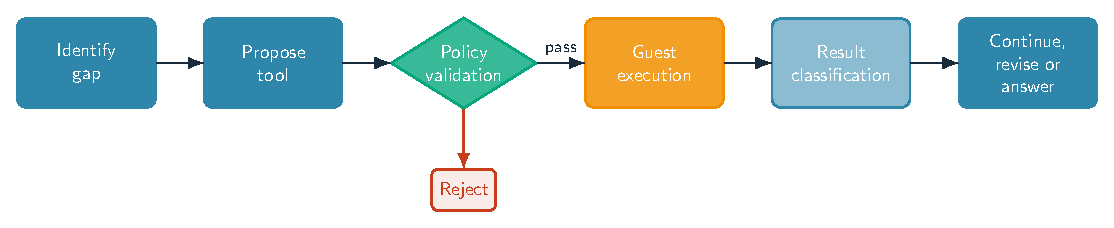
\includegraphics[width=0.95\linewidth]{Figures/fig_dynamic_tool_flow.pdf}
    \caption{Dynamic tool synthesis execution flow, showing the policy gate between tool proposal and guest execution.}
    \label{fig:dynamic_tool_flow}
\end{figure}

\fref{fig:dynamic_tool_flow} captures the six-stage execution loop described above.

\section{Ephemeral Sandboxing}
All executions of dynamic tools for each evaluation session can run in an
ephemeral sandboxed microVM. This creates a barrier to prevent cross-tool
contamination; to prevent persistent state abuse; to prevent memory poisoning.
The host will destroy the guest state after the execution of each evaluation and
store only pre-approved artifacts/logs/benchmark outputs.

A microVM backed task has the following life cycle:
\begin{enumerate}
    \item Allocate/resume guest image.
    \item Establish vsock transport.
    \item Send execution request/input bundle.
    \item Enforce timeout/output limit on host side.
    \item Receive/validate response from guest.
    \item Copy out validated approved artifacts.
    \item Destroy/reset guest state.
\end{enumerate}

For resume from snapshot, if used, reduces the start up time. However, it must be
used with caution. A valid snapshot must represent the original base state prior
to the generation of task specific secret files/tools and/or previous generated
tools. For evaluations that are at risk, use a completely new guest as it will
provide the most clear separation between tasks.

\begin{figure}[htbp]
    \centering
    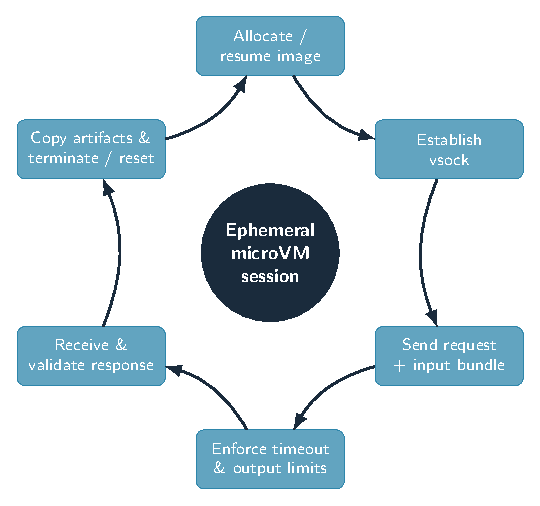
\includegraphics[width=0.8\linewidth]{Figures/fig_microvm_lifecycle.pdf}
    \caption{Lifecycle of an ephemeral microVM-backed tool execution session.}
    \label{fig:microvm_lifecycle}
\end{figure}

\fref{fig:microvm_lifecycle} shows the lifecycle of an ephemeral session.

The Host Daemon, Guest Runtime, Protocol Boundary, Dynamic Execution Engine,
MicroVM Lifecycle, Policy Model, and Failure-Handling Strategy are all defined in
this chapter. In the next chapter we will describe the evaluation method for the
system.

\section{Failure Modeling}
The failures that occur during the operation of the micro-vm are a key part of how ironclaw operates. Therefore when generating tools for the user they can fail to compile; time-out; generate incorrect results (provide invalid output); or attempt to execute malicious code. For every type of failure ironclaw will capture the specific failure classification with respect to the tool being executed, so the next process is done without exposing the host to the risk associated with that particular failure.

\section{Operational Considerations}
In addition to tracking which application was requested based on the unique id of the request; what policy decision was made at that time; what the duration of the execution was; what the final exit status was of the last task executed; and whether there were any truncations in the output. The guest should not log anything but information related to executing tasks. Also the guest should not have access to any secret information from the host. All this information is helpful for debugging; benchmarking; and security audits; none of them would violate the isolation boundaries.
